\documentclass[12pt,a4paper]{report}
\usepackage{natbib}%referencing
\usepackage[left=1.0in,right=1.0in,top=0.8in,bottom=0.8in]{geometry}
\usepackage{float}
\linespread{1.3}
\usepackage{graphicx}%figures
\usepackage{fancyhdr}
\pagestyle{fancyplain}
\fancyhf{}
\fancyfoot[C]{\thepage}
\fancyhead[R]{\large{Title of the project}}%project title
\renewcommand{\headrulewidth}{0pt}
\usepackage{rotating}%landscape image
\usepackage{amsmath}%math
\usepackage{titlesec} %formatting chapters
%\titlespacing*{<command>}{<left>}{<before-sep>}{<after-sep>}
\titlespacing*{\chapter}{-15pt}{10pt}{15pt}
\titlespacing*{\section}{0pt}{0pt}{5pt}
\titlespacing*{\subsection}{0pt}{5pt}{5pt}
\titleformat{\chapter}[hang] 
{\normalfont\huge\bfseries}{\chaptertitlename\ \thechapter.}{1em}{\centering}
\renewcommand{\chaptername}{}
\graphicspath{{Images/}}%image folder name
%Cover page contents
\title{
\large{
    \textbf{AN ENGINEERING PROJECT REPORT}\\
    {On}\\
    \textbf{TITLE OF THE PROJECT}\\
    \vspace{.7cm}
    {\textbf{Submitted By}\\
    Full Name \hspace{1cm}Class Roll\\
    Full Name \hspace{1cm}Class Roll\\
    Full Name \hspace{1cm}Class Roll\\
    Full Name \hspace{1cm}Class Roll\\}
    \vspace{.7cm}
    {\textbf{Submitted To}\\
    The Department of Information and Communications Technology\\
    in partial fulfillment of requirement for the degree of Bachelor of Engineering in ........}\\
    \vspace{.7cm}
    {
\includegraphics[scale=.2]{logo.png}}\\
    \vspace{.7cm}
    \textbf{Cosmos College of Management \& Technology\\
    (Affiliated to Pokhara University)\\
    Tutepani, Lalitpur, Nepal}
        }
    }
\date{May, 2022} %{Month Year}

\begin{document}
\maketitle
\newpage
\begin{center}
\large{
    \textbf{AN ENGINEERING PROJECT REPORT}\\
    {On}\\
    \textbf{TITLE OF THE PROJECT}\\
    \vspace{.7cm}
    {\textbf{Submitted By}\\
    Full Name \hspace{1cm}Class Roll\\
    Full Name \hspace{1cm}Class Roll\\
    Full Name \hspace{1cm}Class Roll\\
    Full Name \hspace{1cm}Class Roll\\}
    \vspace{.7cm}
    \textbf{Under the Supervision of}\\
    NAME OF SUPERVISOR\\
    \vspace{.7cm}
    {\textbf{Submitted To}\\
    The Department of Information and Communications Technology\\
    in partial fulfillment of requirement for the degree of Bachelor of Engineering in ........}\\
    \vspace{.7cm}
    {
\includegraphics[scale=.2]{logo.png}}\\
    \vspace{.7cm}
    \textbf{Cosmos College of Management \& Technology\\
    (Affiliated to Pokhara University)\\
    Tutepani, Lalitpur, Nepal}
        }
\vspace{70pt}\\
{May, 2022} %{Month Year}
\end{center}
\pagenumbering{roman}
\setcounter{page}{2}
\newpage
\chapter*{Copyright}
\addcontentsline{toc}{chapter}{\numberline{}Copyright}
The author has agreed that the Library, University of Pokhara, Cosmos College of Management \& Technology, May make this engineering project report freely available for inspection, Moreover, the author has agreed that permission for extensive copying of this report for scholarly purpose may be granted by the supervisor who supervised the work recorded here in or, in their absence, by the college authority in which the project work was done. Copying or any other use of this report for financial gain without approval of the college and author’s permission is strictly prohibited.\\
Request for the permission to copy or to make and other use of the materials in this report in the whole or in part should be addressed to:
\vspace{50pt}\\
Cosmos College of Management \& Technology\\
©Copyright 2022
%new chapter
\chapter*{Certificate}
\addcontentsline{toc}{chapter}{\numberline{}Certificate}
\vspace{20pt}
The undersigned certify that they have read \& recommended to the Department of Electronics \& Communication \ IT \& Computer \ Civil, a final year project work entitled “The Title of the Project Work” submitted by (Names of the Students with Roll Numbers) in partial fulfillment of the requirements for the degree of Bachelor of Engineering.\\
\vspace{60pt}\\
----------------------------------\\
\textbf{Name \& Post of Project Supervisor}\\
(Project Supervisor)\\
Department of ………….\\
Name of Institute\\
\newline
\newline
----------------------------------\\
\textbf{Name External Examiner}\\
(External Examiner)\\
Designation\\
Name of Institute\\
\newline
\newline
----------------------------------\\
\textbf{Name}\\
Head of the Department\\
Department of IT and Computer Engineering\\
Cosmos College of Management and Technology\\
%new chapter
\chapter*{Acknowledgments}
\addcontentsline{toc}{chapter}{\numberline{}Acknowledgements}
On this page, the author expresses his gratitude and concern by using praising and thanksgiving words.  don’t forget to include your project supervisor name.
%new chapter
\chapter*{Abstract}
Abstract represents a summarized report of the complete project in a very concise and informative format followed with 3 to 5 keywords (italic). The entire abstract of a project report should be written in about 250 to 350 words.\\
\newline
Keywords: \textit{keyword 1, keyword 2, keyword 3,keyword 4, Keyword 5}
\addcontentsline{toc}{chapter}{\numberline{}Abstract}
\tableofcontents
\addcontentsline{toc}{chapter}{\numberline{}Contents}
\listoffigures
\addcontentsline{toc}{chapter}{\numberline{}List of Figures}
\listoftables
\addcontentsline{toc}{chapter}{\numberline{}List of Tables}
\chapter*{List of Abbreviations}
\addcontentsline{toc}{chapter}{\numberline{}List of Abbreviations}
\begin{tabular}{c l}
\textbf{LAH}     &  List of Abbreviations Here\\
\textbf{AMC}     &  Add More Contents
\end{tabular}
% Latex instruction starts here
\chapter{This Chapter is for Latex Guidelines}
\section{Introduction to \LaTeX}
Welcome to this \LaTeX Report Template, a beautiful and easy to use template for writing a report using the \LaTeX typesetting system.
\section{Tables}
%table 1
\begin{table}[H]% place table here
\centering
    \caption{\textbf{Table style 1}} %this is caption, usually place above the table
    \vspace{8pt} %puts 8pt vertical space after caption
\begin{tabular}{|c|c|c|c|} % table with 4 columns, c for centered other options l'left' r'right'
\hline%insert hosizontal line
\textbf{Roll No} & \textbf{Name} & \textbf{Address} & \textbf{Score in \%} \\ \hline
101 & Bishwas Pokheral & Morang & 92 \%\\ \hline
102 & Aashish Yadav    & Siraha & 89 \%\\ \hline
\end{tabular}
\end{table}
%Table 2
\begin{table}[H]
\centering
    \caption{\textbf{Table style 2}}
    \vspace{8pt} %puts 8pt vertical space after caption
\begin{tabular}{cccc} % table with 4 columns, c for centered other options l'left' r'right'
\hline%insert hosizontal line
\textbf{Roll No} & \textbf{Name} & \textbf{Address} & \textbf{Score in \%} \\ \hline
101 & Bishwas Pokheral & Morang & 92 \%\\ 
102 & Aashish Yadav    & Siraha & 89 \%\\ \hline
\end{tabular}
\end{table}
\section{Figures}
%normal figures
\begin{figure}[H]
    \centering
    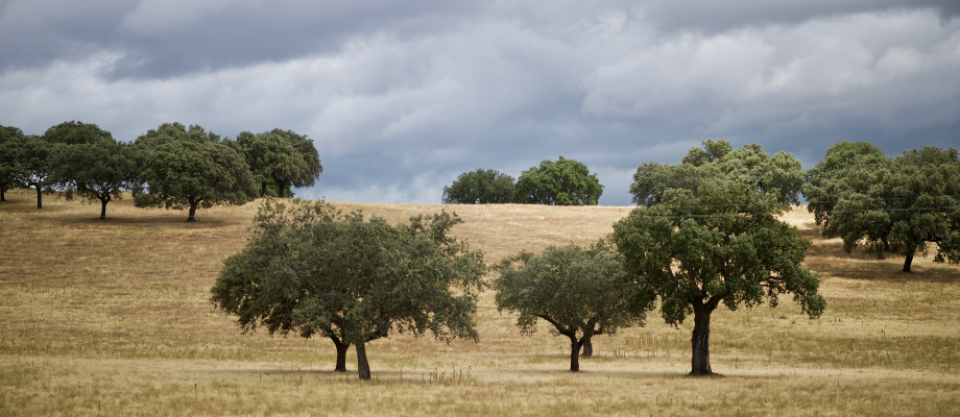
\includegraphics[width=\textwidth,height=3in,scale=0.5]{fig.png}
    \caption{The image is scaled to a width that will just fit within the margins. After that scale the graphics to the specified height i.e. 3 inch and scale graphics by scale factor 0.5 i.e. makes the graphic half the original size.}
\end{figure}
%landscape figure
\begin{sidewaysfigure}[]
\centering
    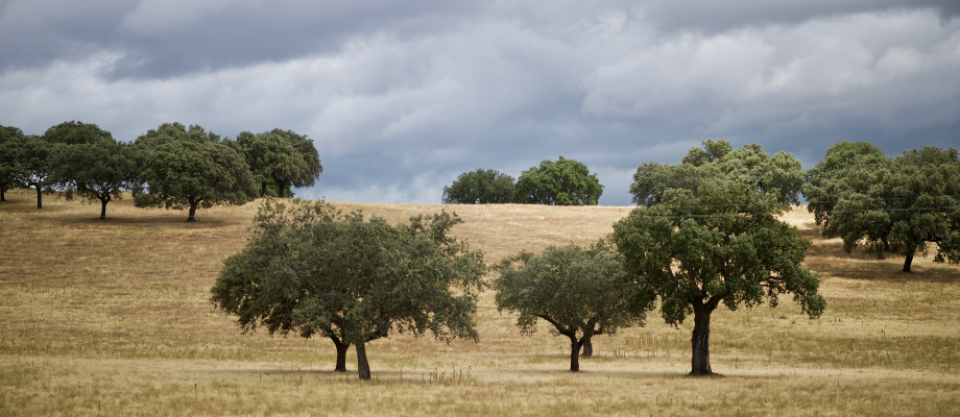
\includegraphics[width=\textwidth]{fig.png}
    \caption{Caption in landscape to a figure in landscape.}
    \label{fig:LandscapeFigure}
\end{sidewaysfigure}
%rotate figure
\begin{figure}[H]
    \centering
    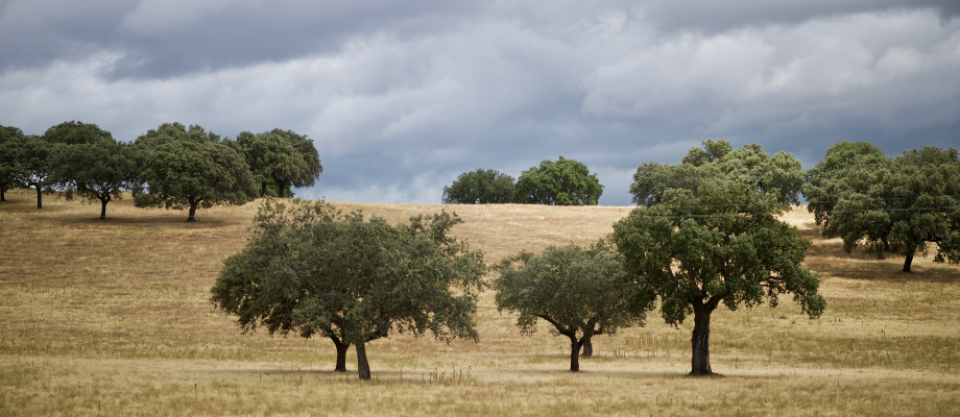
\includegraphics[angle=45,width=\textwidth,height=3in,scale=0.5]{fig.png}
    \caption{The image is rotated counter-clockwise by 45 degree and other parameters same as above figure.}
\end{figure}
\section{Mathematics}
\begin{figure}[H]
    \centering
    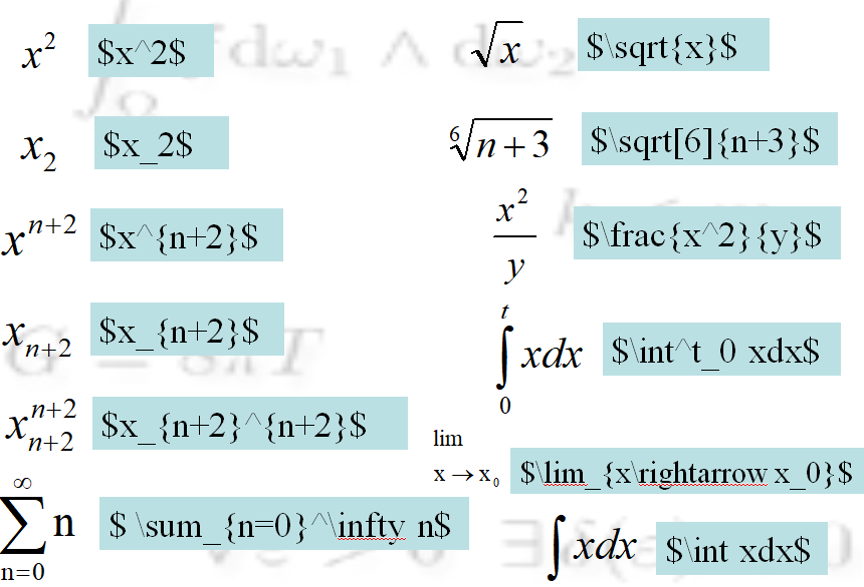
\includegraphics[width=\textwidth]{math.png}
\end{figure}
\subsection{Equation environment}
This environment is used for numbered equation\\
\textbf{Example:}\\
The derivative of the function $f(x)$ at the point $x_0$ is
\begin{equation}
f'(x_0) =
\lim_{x \rightarrow x_0}
\frac{f(x) - f(x_0)}{x - x_0}
\end{equation}
\subsection{Eqnarray Environment}
This environment is used for multiple column numbered equations. Include the command \verb!\nonumber! on any line to suppress the equation number.\\
\textbf{Example}\\
\begin{eqnarray}
(a + b)(a + b) & = & a^2 + ab + ba + b^2 
\nonumber \\
& = & a^2 + 2ab + b^2 \\
(a + b)(a - b) & = & a^2 - ab + ba - b^2
\nonumber \\
& = & a^2 - b^2\\
(a + b)^3 & = & a^3 + 3a^2b + 3ab^2 + b^3 
\end{eqnarray}
\subsection{Array environment for matrix!}
\begin{equation}
A=\left[
\begin{array}{cccc}
a_{1,1} & a_{1,2} & \ldots & a_{1,n}\\
a_{2,1} & a_{2,2} & \ldots & a_{2,n}\\
\vdots  & \vdots  & \ddots & \vdots \\
a_{m,1} & a_{m,2} & \ldots & a_{m,n}
\end{array}
\right]
\end{equation}
\section{Referencing}
\begin{itemize}
    \item First include package for referencing as \verb!\usepackage{natbib}! 
    \item Then, we create a file whose name ends with the extension .bib ‘filename.bib’ that holds all the sources for referencing.
    \item The entries in your ‘.bib file’ are called in your LATEX file with \verb!\cite! commands as: \verb!\cite{source_name}!
    \item After that, in your LATEX file, you provide just two more pieces of information:
    \begin{itemize}
        \item A \verb!bibliographystyle{style_name}! command to specify the formatting style of the citations
        \item The \verb!\bibliography{file_name}! at the point you want the bibliography printed.
    \end{itemize}
\end{itemize}
% instruction ends here
\chapter{Introduction}
\pagenumbering{arabic}%start arabic numbering(1,2,3..) from here
\fancyhf{}
\fancyhead[R]{\large{Title of the project}}%project title
\fancyfoot[R]{\thepage}
This chapter should contain brief background information and overview about the project, the problem-statement, scope \& objective the project. It rarely contains drawings and graphical illustrations.
\section{Background}
\section{Rationale}
\section{Statements of the Problems}
\section{Objectives}
\chapter{Literature Review}
\chapter{Requirement Analysis}
\section{Feasibility Study}
\section{Functional and Non Functional Requirements}
\section{Hardware and Software Requirements}
\section{Tools and Environments}
\chapter{Methodology}
\section{Software Process Model}
\section{Algorithms / Working Principle}
\section{Block Diagram of Proposed System}
\section{UML Diagrams}
\subsection{Use Case}
\subsection{Sequence}
\subsection{Activity etc.}
\section{Data Sets (optional)}
\section{Validation (optional)}
\chapter{Results \& Discussion}
\chapter{Limitations and Future Enhancement}
\chapter{Conclusion}
The conclusion part summarizes the whole report by highlighting all the chapters and their significance and the importance of the project and the achievements.
\chapter{Limitations and Future enhancement}
This chapter should contains major limitations of the project and the further enhancement of the project in near future with different but related approach. \textbf{Referencing checking here}\cite{giri2019transfer}
\addcontentsline{toc}{section}{References}
\renewcommand{\bibname}{References}
\bibliographystyle{unsrt}
\bibliography{refs}
\chapter*{Appendices}
\addcontentsline{toc}{section}{Appendices}
\section*{Screenshots}
\section*{Complete Circuit Diagram}
\section*{PCB Diagrams ( If Any)}
\section*{Data-sheets (only of special components used – if any)}
\end{document}
